 	 \section{Introduction}
 	  
    
    Le cloud computing, traduit le plus souvent en français par " informatique dans les nuages", " informatique dématérialisée " ou encore " infonuagique ", est un domaine qui regroupe un ensemble de techniques et de pratiques consistant à accéder, en libre-service, à du matériel ou à des logiciels informatiques, à travers une infrastructure réseau (Internet). Ce concept rend possible la distribution des ressources informatiques sous forme de services pour lesquels l'utilisateur paie uniquement pour ce qu'il utilise. Ces services peuvent être utilisés pour exécuter des applications scientifiques et commerciales, souvent modélisées sous forme de workflows.
     
    Ce chapitre présente une introduction au cloud computing et au workflow, nécessaire pour la compréhension générale de ce rapport.
    
    Tout d’abord, nous présentons dans la section 1.2 une introduction au paradigme du cloud computing. Nous donnons un aperçu général du cloud computing, y compris sa définition, ses caractéristiques principales et une comparaison avec les technologies connexes. Nous présentons les différents modèles de service, les différents modèles de déploiement, ainsi que les différents acteurs du cloud computing. Nous résumons quelques challenges de recherche en cloud computing. Par la suite, nous présentons, dans la section 1.3, une introduction au workflow et systèmes de gestion de workflow. Nous donnons le concept du workflow, sa définition, et l’architecture de référence d’un système de gestion de workflows et, finalement, nous résumons l'intérêt du cloud pour les workflows.
    
    \section{cloud computing}
    \subsection{Concept du cloud computing}
  L’idée principale du cloud est apparue dans les années 60, où le professeur John McCarthy avait imaginé que les ressources informatiques seront fournies comme des services d’utilité publique (Garfinkel, 1999). C'est ensuite, vers la fin des années 90, que ce concept a pris de l'importance avec l’avènement du grid computing  (Foster, 1999). Le terme cloud est une métaphore exprimant la similarité avec le réseau électrique, dans lequel l'électricité est produite dans de grandes centrales, puis disséminée à travers un réseau jusqu'aux utilisateurs finaux. Ici, les grandes centrales sont les Datacenter, le réseau est le plus souvent celui d'Internet et l'électricité correspond aux ressources informatiques. Le cloud computing  n'est véritablement apparu qu'au cours de l’année 2006 (Vouk, 2008) avec l'apparition d'Amazon EC2 (Elastic Compute cloud). C'est en 2009 que la réelle explosion du cloud survint avec l'arrivée sur le marché de sociétés comme Google (Google App Engine), Microsoft (Microsoft Azure), IBM (IBM Smart Business Service), Sun (Sun cloud) et Canonical Ltd (Ubuntu Enterprise cloud). D'après une étude menée par Forrester (Ried, 2011), le marché du cloud computing  s'élevait à environ 5,5 milliards de dollars en 2008, il devrait atteindre plus de 150 milliards d'ici 2020, comme l’illustre la figure \ref{fig:tempsnip4}. 
    
    \begin{figure}[h]
    	\centering
    	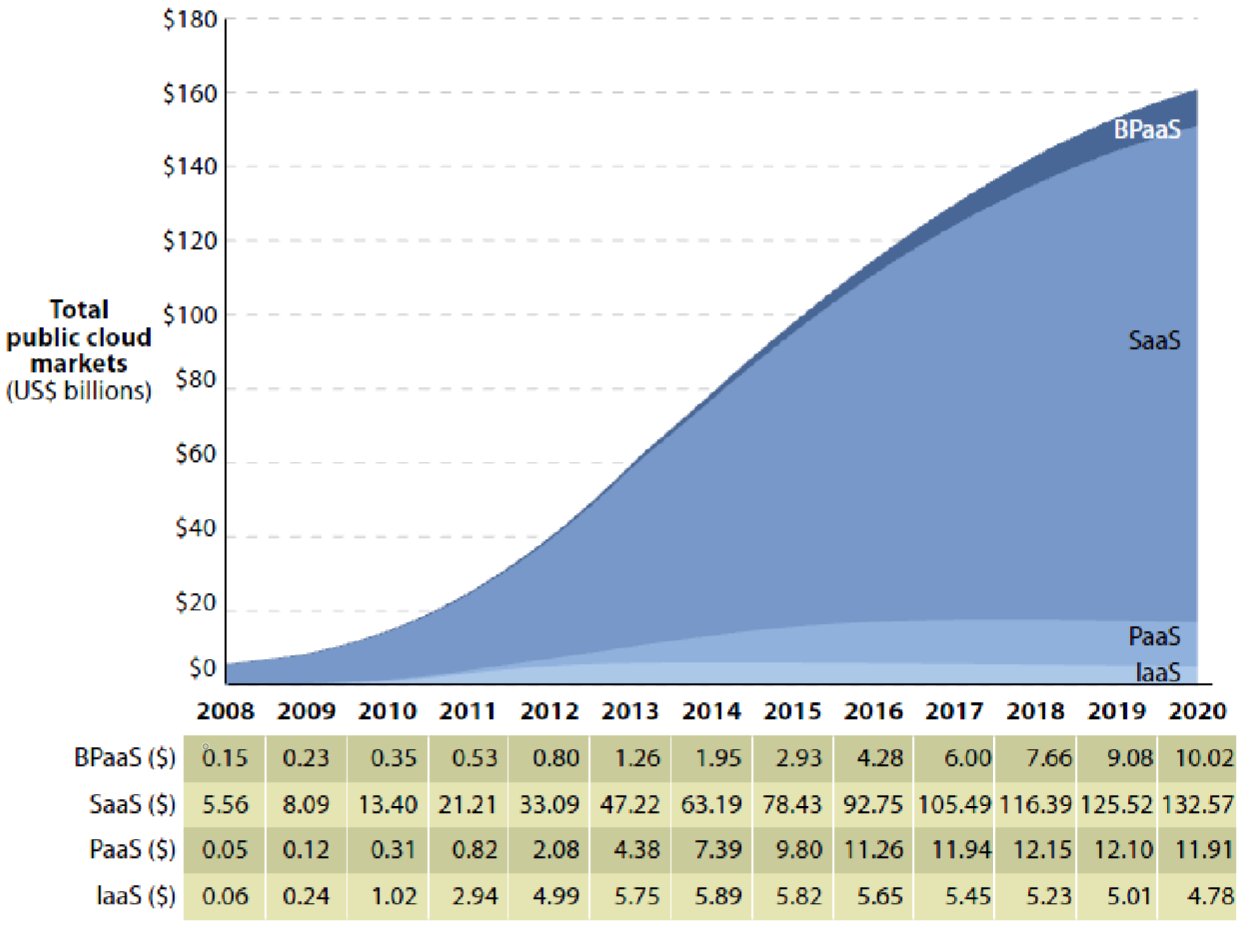
\includegraphics[width=0.7\linewidth]{images/tempsnip4}
    	\caption{Prévisions de la taille du marché du cloud computing  public (Ried, 2011).}
    	\label{fig:tempsnip4}
    \end{figure}
\subsubsection{Vers une définition du cloud computing }
Beaucoup de chercheurs ont tenté de définir le cloud computing (Geelan, 2008 ; McFedries, 2008 ; Buyya, 2009 ; Armbrust, 2010). La plupart des définitions attribuées à ce concept semblent se concentrer seulement sur certains aspects technologiques. L'absence d'une définition standard a généré non seulement des exagérations du marché, mais aussi des confusions. Pour cette raison, il y a eu récemment des travaux sur la normalisation de la définition du cloud computing, à l'exemple de Vaquero et coll (Vaquero, 2009) qui ont comparé plus de 20 définitions différentes et ont proposé une définition globale.  En guise de synthèse des différentes propositions données dans la littérature, nous introduisons une définition mixte, qui correspond aux différents types de cloud considérés dans les travaux réalisés dans cette thèse.

  Nous définissons le cloud comme un modèle informatique qui permet d’accéder, d’une façon transparente et à la demande, à un pool de ressources hétérogènes physiques ou virtualisées (serveurs, stockage, applications et services) à travers le réseau. Ces ressources sont délivrées sous forme de services reconfigurables et élastiques, à base d’un modèle de paiement à l’usage, dont les garanties sont offertes par le fournisseur via des contrats de niveau de service (SLA, Service Level Agreement).     

    \subsubsection{Caractéristiques principales du cloud computing}
    Le cloud computing  possède les caractéristiques suivantes :
    \begin{itemize}
    	\item 	\textbf{Accès en libre-service à la demande}. Le cloud computing offre des ressources et services aux utilisateurs à la demande. Les services sont fournis de façon automatique, sans nécessiter d’interaction humaine (Mell, 2011). 
    \item	\textbf{Accès réseau universel.}  Les services de cloud computing  sont facilement accessibles au travers du réseau, par le biais de mécanismes standard, qui permettent une utilisation depuis de multiples types de terminaux (par exemple, les ordinateur portables, tablettes, smartphones) (Mell, 2011). 
   \item \textbf{Mutualisation de ressources} (Pooling). Les ressources du cloud peuvent être regroupées pour servir des utilisateurs multiples, pour lesquels des ressources physiques et virtuelles sont automatiquement attribuées (Mell, 2011). En général, les utilisateurs n’ont aucun contrôle ou connaissance sur l’emplacement exact des ressources fournies. Toutefois, ils peuvent imposer de spécifier l’emplacement à un niveau d’abstraction plus haut.
   \item \textbf{Scalabilité et élasticité.} Des ressources supplémentaires peuvent être automatiquement mises à disposition des utilisateurs en cas d’accroissement de la demande (en réponse à l'augmentation des charges des applications) (Geelan, 2008), et peuvent être libérées lorsqu’elles ne sont plus nécessaires. L’utilisateur a l’illusion d’avoir accès à des ressources illimitées à n'importe quel moment, bien que le fournisseur en définisse généralement un seuil (par exemple : 20 instances par zone est le maximum possible pour Amazon EC2).
   \item \textbf{Autonome.} Le cloud computing  est un système autonome et géré de façon transparente pour les utilisateurs. Le matériel, le logiciel et les données au sein du cloud peuvent être 
    	automatiquement reconfigurés, orchestrés et consolidés en une seule image qui sera fournie à l’utilisateur (Wang, 2008).
    	\item \textbf{Paiement à l’usage.} La consommation des ressources dans le cloud s’adapte au plus près aux besoins de l’utilisateur. Le fournisseur est capable de mesurer de façon précise la consommation (en durée et en quantité) des différents services (CPU, stockage, bande passante,…) ; cela lui permettra de facturer l’utilisateur selon sa réelle consommation (Armbrust, 2009). 
    	\item \textbf{Fiabilité et tolérance aux pannes.} Les environnements cloud tirent parti de la redondance intégrée du grand nombre de serveurs qui les composent en permettant des niveaux élevés de disponibilité et de fiabilité pour les applications qui peuvent en bénéficier (Buyya, 2008). 
    	\item \textbf{Garantie QoS.} Les environnements de cloud peuvent garantir la qualité de service pour les utilisateurs, par exemple, la performance du matériel, comme la bande passante du processeur et la taille de la mémoire (Wang, 2008). 
    	\item \textbf{Basé-SLA.} Les clouds sont gérés dynamiquement en fonction des contrats d’accord de niveau de service (SLA) (Buyya, 2008) entre le fournisseur et l’utilisateur. Le SLA définit des politiques, telles que les paramètres de livraison, les niveaux de disponibilité, la maintenabilité, la performance, l'exploitation, ou autres attributs du service, comme la facturation, et même des sanctions en cas de violation du contrat. Le SLA permet de rassurer les utilisateurs dans leur idée de déplacer leurs activités vers le cloud, en fournissant des garanties de QoS. 
    	Après avoir présenté les caractéristiques essentielles d’un service cloud, nous présentons, brièvement, dans la section suivante, quelques technologies connexes aux clouds.
    	
    \end{itemize} 
\subsubsection{Technologies connexes }

\subsection{Modèles du cloud computing  }
\subsubsection {Modèles de service du cloudcomputing}  
XaaS (X as a Service) représente la base du paradigme du cloud computing, où X représente un service tel qu’un logiciel, une plateforme, une infrastructure, un Business Process, etc. Nous présentons, dans cette section,  quatre  modèles de services (Rimal, 2009), à savoir: (1) Logiciel en tant que services SaaS (Software as a Service), où le matériel, l’hébergement, le framework d’application et le logiciel sont dématérialisés, (2) Plateforme en tant que service PaaS (Platform as a Service), où le matériel, l’hébergement et le framework d’application sont dématérialisés, (3) Infrastructure en tant que service IaaS (Infrastructure as a Service) et (4) Matériel en tant que service HaaS (Hardware as a Service), où seul le matériel (serveurs) est dématérialisé dans ces deux derniers cas. La figure \ref{fig:capture5} montre le modèle classique et les différents modèles de service de cloud
\begin{figure}[h]
	\centering
	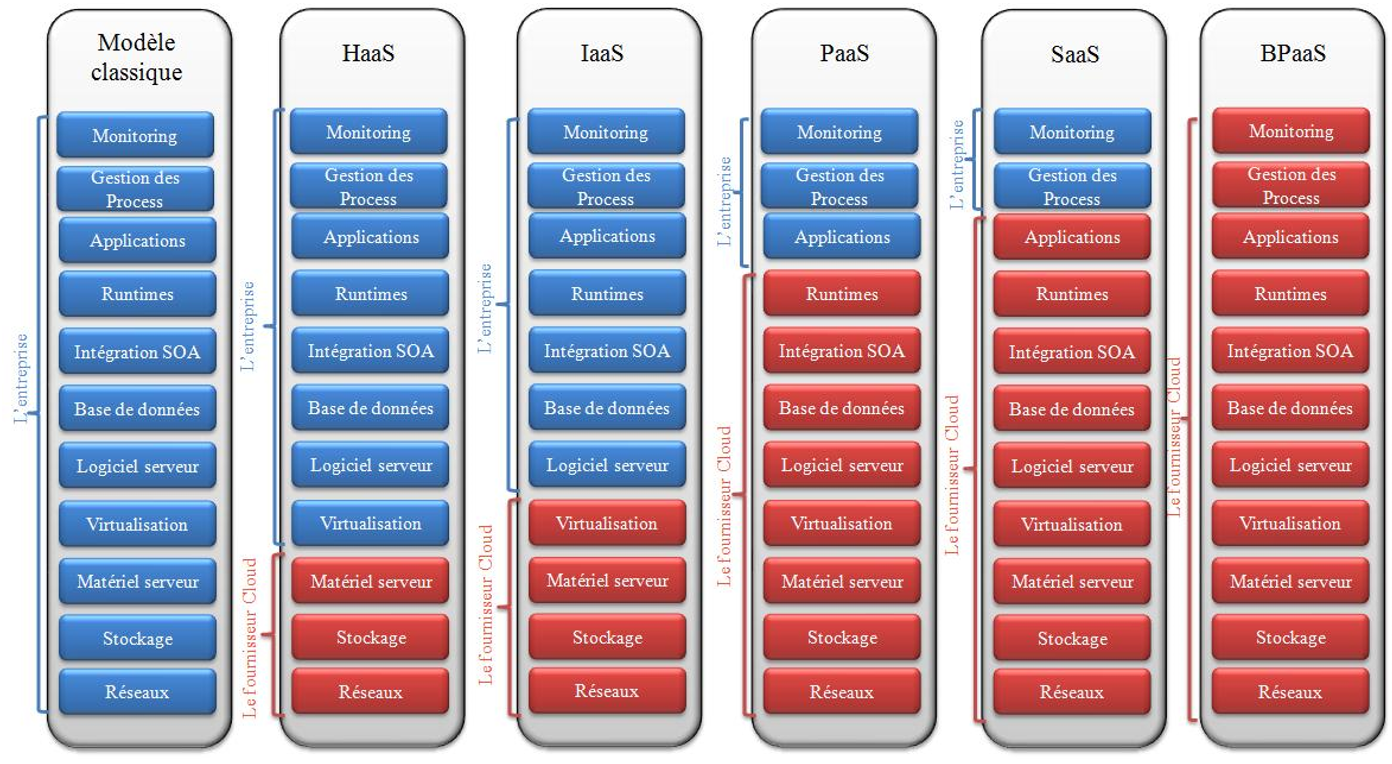
\includegraphics[width=0.7\linewidth]{Capture5}
	\caption{Les services XaaS du cloud computing}
	\label{fig:capture5}
\end{figure}

\begin{enumerate}
\item 	\textbf{Software as a Service (SaaS):}

Ce modèle de service est caractérisé par l’utilisation d’une application partagée qui fonctionne sur une infrastructure Cloud. L’utilisateur accède à l’application par le réseau au travers de divers types de terminaux (souvent via un navigateur web). L’administrateur de l’application ne gère pas et ne contrôle pas l’infrastructure sous-jacente (réseaux, serveurs, applications, stockage).  Il ne contrôle pas les fonctions de l’application à l’exception d’un paramétrage de quelques fonctions utilisateurs limitées. On prend comme exemple les logiciels de messagerie au travers d’un navigateur comme Gmail ou Yahoo mail. 

\item  \textbf{ Platform as a Service (PaaS):}

L’utilisateur a la possibilité de créer et de déployer sur une infrastructure Cloud PaaS ses propres applications en utilisant les langages et les outils du fournisseur. L’utilisateur ne gère pas ou ne contrôle pas l’infrastructure Cloud sous-jacente (réseaux, serveurs, stockage) mais l’utilisateur contrôle l’application déployée et sa configuration. Comme exemple de PaaS, on peut citer un des plus anciens -IntuitQuickbase- qui permet de déployer ses applications bases de données en ligne ou -Google Apps Engine (GAE)- pour déployer des services Web. 

Dans ces deux cas l’utilisateur de ces services n’a pas à gérer des serveurs ou des systèmes pour déployer ses applications en ligne et dimensionner des ressources adaptées au trafic.
\item   \textbf{Infrastructure as a Service (IaaS):}

L’utilisateur loue des moyens de calcul et de stockage, des capacités réseau et d’autres ressources indispensables (partage de charge, pare-feu, cache). L’utilisateur a la possibilité de déployer n’importe quel type de logiciel incluant les systèmes d’exploitation. L’utilisateur ne gère pas ou ne contrôle pas l’infrastructure Cloud sous-jacente mais il a le contrôle sur les systèmes d’exploitation, le stockage et les applications. Il peut aussi choisir les caractéristiques principales des équipements réseau comme le partage de charge, les pare-feu, etc. L’exemple emblématique de ce type de service est Amazon Web Services qui fournit du calcul (EC2), du stockage (S3, EBS), des bases de données en ligne (SimpleDB) et quantité d’autres services de base. Il est maintenant imité par de très nombreux fournisseurs.
	\item \textbf{Points fortset Points faibles des services cloud:} 
\end{enumerate}
\subsubsection { Modèles de déploiement}  

Selon la définition du cloud computing  donnée part le NIST (Mell, 2011), il existe quatre modèles de déploiement des services de cloud, à savoir : cloud privé, cloud communautaire, cloud public et cloud hybride, comme illustré dans la figure \ref{fig:cloudmd}.
\begin{enumerate}
	\item \textbf{Cloud privé :}\\
	 L’ensemble des ressources d’un cloud privé est exclusivement mis à disposition d’une entreprise ou organisation unique. Le cloud privé peut être géré par l’entreprise ellemême (cloud privé interne) ou par une tierce partie (cloud privé externe). Les ressources d’un cloud privé se trouvent généralement dans les locaux de l’entreprise ou bien chez un fournisseur de services. Dans ce dernier cas, l’infrastructure est entièrement dédiée à l’entreprise et y est accessible via un réseau sécurisé (de type VPN).  L’utilisation d’un cloud privé permet de 	garantir, par exemple, que les ressources matérielles allouées ne seront jamais partagées par deux clients différents. 
	
	\item \textbf{Cloud communautaire:}\\
	 L’infrastructure d’un cloud communautaire est partagée par plusieurs organisations indépendantes ayant des intérêts communs. L’infrastructure peut être gérée par les organisations membres ou par un tiers. L’infrastructure peut être située, soit au sein des dites organisations, soit chez un fournisseur de services. 
	\item \textbf{Cloud public:}\\
	L’infrastructure d’un cloud public est accessible à un large public et appartient à un fournisseur de services. Ce dernier facture les utilisateurs selon la consommation et garantit la disponibilité des services via des contrats SLA. 
	\item \textbf{Cloud hybride:}\\
	 L’infrastructure d’un cloud hybride est une composition de plusieurs clouds (privé, communautaire ou public). Les différents clouds composant l’infrastructure restent des entités uniques, mais sont reliés par une technologie standard ou propriétaire permettant ainsi la portabilité des données ou des applications déployées sur les différents clouds.  

\begin{figure}[h]
	\centering
	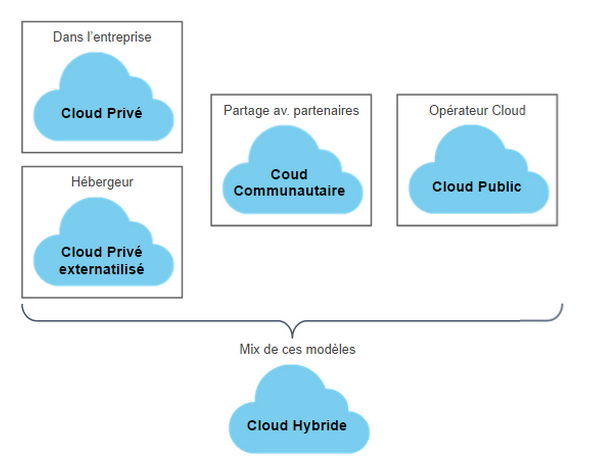
\includegraphics[width=0.5\linewidth]{Cloud_MD}
	\caption{Modèles de déploiement du cloud computing }
	\label{fig:cloudmd}
\end{figure}
\end{enumerate}

\subsection{Cloud computing et sécurité
}
Toutes les enquêtes montrent que la sécurité est la préoccupation majeure des organisations dans le processus d’adoption des technologies Cloud. Les questions sont nombreuses comme par exemple :

\begin{itemize}

\item Quelle confiance peut-on avoir dans le stockage des données à l’extérieur de l’entreprise ?
\item Quels sont les risques associés à l’utilisation de services partagés ?
\item Comment démontrer la conformité des systèmes à des normes d’exploitation ?
\end{itemize}

Les infrastructures Cloud sont de gigantesques systèmes complexes. Ils peuvent cependant être réduits à un petit nombre de primitives simples qui sont instanciées des milliers de fois et à quelques fonctions communes. La sécurité du Cloud est donc un problème gouvernable moins complexe qu’il n’y parait.

\subsubsection{Avantages et défis du Cloud en terme de sécurité}

Le Cloud présente des avantages immédiats. D’une manière générale, le fait d’héberger des données publiques sur le Cloud réduit les risques pour les données internes sensibles. D’autre part, l’homogénéité dans la construction du Cloud en rend les tests et les audits plus simples. De même la conduite du système au travers de web services permet la mise en place  de procédures automatiques accroissant notablement la sécurité.

En revanche les défis restent nombreux pour les fournisseurs.  Il faut donner confiance dans le modèle de sécurité et dans les outils de gestion qui sont proposés. Les tâches de gestion sont réalisées de manière indirecte au travers d’une interface puisque l’utilisateur n’a pas de contrôle direct sur l’infrastructure physique. Ce partage des responsabilités complique un peu les audits de sécurité.

\subsubsection{Les composants sécurité d’un système de Cloud computing}
Les différents composants qui participent à la sécurité d’un système de Cloud computing présentent les caractéristiques suivantes :
\begin{itemize}
	 
\item \textbf{Service de console de gestion (Provisioning):}\\
La mise en route et la reconfiguration des composants des systèmes sont très rapides. Il est possible de mettre en service plusieurs instances dans plusieurs centres de traitement répartis dans le monde en quelques minutes. Les reconfigurations réseau sont facilitées. En revanche, la sécurité d’utilisation de la console de gestion devient impérative (authentification multi-facteurs, connexion chiffrée, etc..)

\item \textbf{Service de stockage des données:}\\
Les avantages du stockage des données dans le Cloud dépendent des fournisseurs mais en général, ceux-ci fragmentent et répartissent les données. Celles ci sont aussi souvent recopiées dans des centres de traitement différents. Ces opérations améliorent considérablement la sécurité des données. Si leur contenu doit rester confidentiel, il convient de les chiffrer avant de les stocker.

\item \textbf{Infrastructures de calcul:}\\
Un des gros avantages du Cloud pour le développement et l’exploitation des applications réside dans la virtualisation. Elle permet de préparer des configurations maîtres sûres qu’il suffit de dupliquer pour déployer. Les défis restent la sécurisation des données dans les applications partagées et  la sécurité entre les instances garantie par les hyperviseurs.
\item \textbf{Services de support:}\\
La principale caractéristique du Cloud est la mise en place a priori d’une sécurité renforcée et auditable (authentification, logs, pare-feux, etc..). Il reste à traiter les risques liés à l’intégration avec les applications des utilisateurs ainsi que les processus toujours délicats de mises à jour
\item \textbf{Sécurité périmétrique du réseau Cloud:}\\
Ces grandes infrastructures partagées fournissent des moyens de protection au delà des capacités  d’une entreprise normale comme par exemple la protection contre les attaques DDOS (Distributed Denial Of Service). Les mécanismes de sécurité périmétriques sont généralement bien conçus (fournisseur d’identité, authentification, pare-feux , etc..). En revanche, il reste à traiter les sujets liés à la mobilité.

\end{itemize}

%%%%%%%%%%%%%%%%%%%%%%%%%%%%              Workflow et systèmes de gestion de workflows 
%%%%%%%%%%%%%%%%%%%%%%%%%%%%

 \section{Workflow}
 	 
 	 \subsection{Introduction au Workflow }
 	 
 	 
 	 Un Workflow est la modélisation et la gestion assistée par ordinateur de l’accomplissement des tâches composant un processus administratif ou industriel, en interaction avec divers acteurs (humains, logiciels, ou matériels) invoqués [COURTOIS 96]. Outil informatique d’origine industrielle, le Workflow est l’adaptation de la GED24 adjoint de la faculté à gérer l’échange de messages. Le Workflow propose des solutions d’optimisation et de rationalisation des flux d’informations ; que ces informations soient associées à des documents, des procédures ou des messages complémentant les systèmes de gestion électronique de documents et d’informations.
 	 
 	 A l’heure actuelle plus de 250 Systèmes de Gestion de Workflow (WFMS) sont utilisés ou en développement. Cela signifie que le terme « gestion de Workflow » n’est pas simplement une nouvelle expression à la mode. Ce phénomène de gestion de processus (Workflow) aura certainement un fort impact sur la génération suivante de systèmes informatiques [COURTOIS 96, HAYES 91, KOULOPOULOS 95, SCHAEL 97].
 	 
 \subsection{Origines} 
 	 Il est intéressant de considérer l’évolution des systèmes informatiques au cours des quatre dernières décennies [VAN DER AALST 02] pour prendre conscience de la pertinence d’une gestion électronique de processus (Workflow) et apprécier l’impact de la gestion de Workflow dans un avenir proche.
 	 
 	  La Figure \ref{fig:wfmchistory} présente le phénomène de gestion de Workflow dans une perspective historique. Cette figure décrit l’architecture d’un système informatique classique en termes de composants. Dans les années soixante, un système informatique était composé d’un certain nombre d’applications autonomes. Pour chacune de ces applications une interface utilisateur et un système de base de données spécifique étaient développés, chaque application possédait donc ses propres routines pour interagir avec l’utilisateur, stocker et récupérer les données. Dans les années soixante-dix, le développement des systèmes de gestion de base de données (SGBD) a permis d’extraire les données des applications. En utilisant les SGBD, les applications ont ainsi été libérées du fardeau de la gestion de données. Dans les années quatrevingts, l’apparition de systèmes de gestion d’interface utilisateur « User Interface Management Systems » (UIMS) a permis aux développeurs d’application d’extraire l’interaction avec les utilisateurs des applications. Enfin, les années quatre-vingt-dix sont marquées par l’apparition de logiciels de Workflow, permettant aux développeurs d’application d’extraire les procédures de travail des applications. La Figure \ref{fig:wfmchistory} fait apparaître le système de gestion de Workflow comme une composante générique pour représenter et manipuler les processus d’entreprise25. 
 	  
 	  Ainsi, à l’heure actuelle, beaucoup d’organisations commencent à considérer l’utilité d’outils avancés pour soutenir la conception et l’exécution de leurs processus d’entreprise.
 	 
 	 
 	 
\begin{figure}[h]
	\centering
	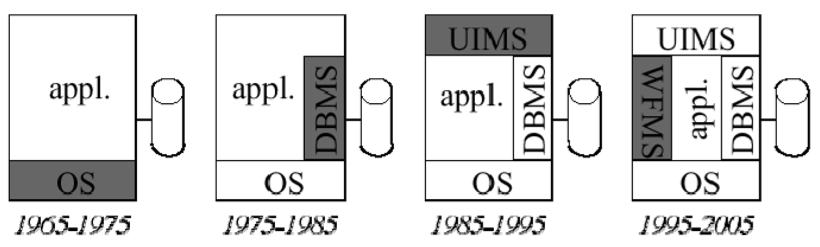
\includegraphics[width=0.7\linewidth]{images/wfmcHistory}
	\caption{Les systèmes de gestion de Workflow dans une perspective historique }
	\label{fig:wfmchistory}
\end{figure}
 	 
 	 
 	 \subsection{Définitions et terminologies }
 	 
 	 Les définitions sont, pour la majorité, issues de la Coalition de Gestion de Workflow « Workflow Management Coalition » (WfMC). La WfMC a été fondée en 1993 par un regroupement d’industriels de l’informatique, de chercheurs et d’utilisateurs, associée à l’essor du développement des Workflows. Cette coalition a pour but de promouvoir les Workflow et d’établir des standards pour les « Workflow Management System » (WfMS). Elle a en particulier publié un glossaire de référence contenant les terminologies employées dans ce domaine [WFMC03 95 ; WFMC11 99]. Ces standards servent notamment à résoudre les problèmes d’interopérabilité entre systèmes Workflow mais également à définir les caractéristiques fondamentales de ces systèmes. Les documents publiés par la WfMC, qui couvrent plusieurs aspects, peuvent être considérés comme des références en la matière. 
 	
 	\subsection{Définitions de base du Workflow } 
 	 
 	 Le sens du mot Workflow peut varier en fonction du contexte. Pour plus de clarté, les définitions les plus communément admises sur les concepts et les termes du Workflow sont rappelées ci dessous. Ces définitions sont principalement issues du « Workflow Management Coalition Terminology and Glossary » WFMC-TC-1011 [WFMC11 99], dont il existe une traduction à usage francophone [WFMC03f 98]. L’idée première du Workflow est donc de séparer les processus, les ressources et les applications, afin de se recentrer sur la logistique des processus travail et non pas sur le contenu des tâches individuelles. Un Workflow est donc le lien entre ces trois domaines comme précise la Figure 13. 
 	 
 	 
 	 
 	 
 	 
 	 
 	 
 	 
 	 
 	 
 	 
 	 \subsubsection{Définition d’un Workflow }
 	 
 	 
 	 Le Workflow est une technologie informatique ayant pour objectif la gestion des processus d’organisations ou d’entreprises : les termes suivants sont également employés pour qualifier cette technologie « Système de Gestion Electronique de Processus », « Gestion de Workflow » ou « Gestion de processus » [COURTOIS 96]. 
 	 
 	 Le Workflow est l’ensemble des moyens mis en œuvre pour automatiser et gérer les processus d’une organisation. Cette gestion est rendue possible par la représentation sous forme d’un modèle, de tout ou partie des processus considérés. Le Workflow doit ensuite transcrire les modèles obtenus en une forme exécutable. Enfin, ces modèles sont exécutés et gérés. Il est ainsi possible de suivre l’évolution de leur état au fil du temps. La gestion de processus inclut également, au cours de l’exécution, la coordination et la synchronisation des différents acteurs des processus en fonction de l’état actuel des modèles.
 	 
 	 Pour résumer, la Gestion de Processus permet donc d’attribuer à chacun et au bon moment, les tâches dont il a la responsabilité et de mettre à disposition les applications, les outils et les informations nécessaires pour leurs réalisations. Dans un contexte d’acteurs humains, le Workflow permet de décharger les acteurs de certaines tâches de gestion administrative, en leur laissant la possibilité de se concentrer sur les contenus des tâches techniques en rapport avec leurs compétences. De plus, le Workflow donne la possibilité d’effectuer une activité de monitoring sur le déroulement des Workflow de l’entreprise, permettant en particulier de connaître, en fonction de la date, l’état des activités, des acteurs, des applications et quelles sont les prochaines activités planifiées. 
 	 
 	 En synthèse, La WfMC présente le Workflow comme l’automatisation d’un processus d’entreprise, en intégralité ou en partie, pendant laquelle on définit les transmissions des documents, de l’information ou des tâches d’un participant à un autre pour agir, selon un jeu de règles procédurales [WFMC11 99]. Un Système Workflow définit, gère et exécute des procédures en exécutant des programmes dont l’ordre d’exécution est prédéfini dans une représentation informatique de la logique de ces procédures - les Workflow [WFMC11 99]. 
 	 
 	 \subsubsection{ Méta Modèle basique }
 	 Le Workflow est basé sur un ensemble de concepts. La WfMC [WFMC11 99] a proposé un méta modèle de Définition de Procédures, qui identifie les concepts de haut niveau dans la Définition de Processus. Ce modèle permet de mieux appréhender les concepts et leurs interrelations. 
 	 
 	 
 	 
 	 
\begin{figure}[h]
	\centering
	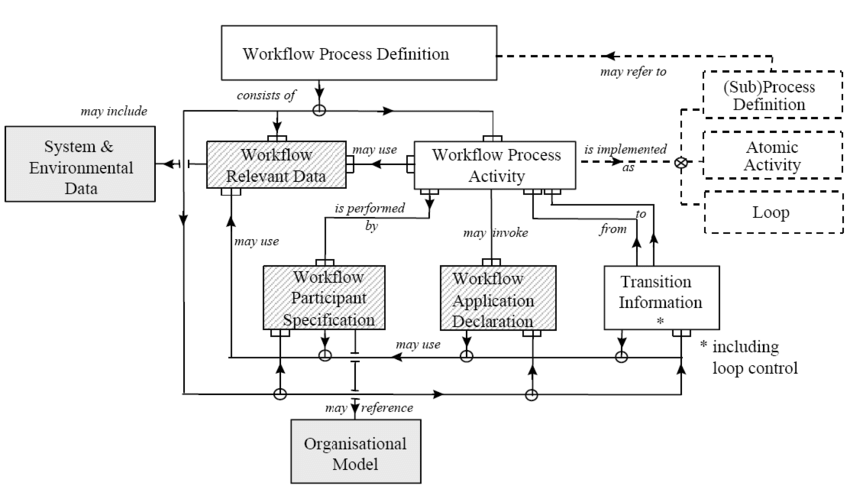
\includegraphics[width=0.7\linewidth]{images/MetaMWFMC11-99}
	\caption{Méta modèle Workflow pour la définition de Processus [WFMC11 99]}
	\label{fig:metamwfmc11-99}
\end{figure}
 	 
 	 Le méta modèle, présenté Figure \ref{fig:metamwfmc11-99}, identifie un ensemble d’objets fondamentaux qui entrent dans la définition d’un processus géré par un système Workflow, et que nous allons définir et commenter dans les paragraphes suivants. Remarquons que le méta modèle peut être enrichi par les développeurs de systèmes, il peut également être utilisé à des fins d’échanges entre différents systèmes Workflow.
 	 
 	\subsection{Concepts et Terminologie Workflow fondamentaux } 
 	 
 	 Les principaux termes associés aux Workflow proposés par la WfMC [WFMC11 99] sont présentés dans le diagramme du méta modèle Workflow ci-dessus, ce diagramme permet également de mettre en évidence leurs interrelations. Les termes présentés ci-dessous en français avec la traduction anglaise originale associée, couvrent les notions plus importantes appartenant au Workflow et à son lexique [WFMC11 99]. 
 	 
 	 \subsubsection{Procédure Workflow (Workflow Process) }
 	 
 	 Une procédure Workflow est une procédure contrôlée par un Workflow. Une procédure est composée de plusieurs activités enchaînées pour représenter un flux de travail. Une procédure possède une structure hiérarchique et modulaire, en l’occurrence une procédure peut donc être composée de sous procédures et d’activités. Les sous-procédures peuvent être composée elles mêmes de procédures manuelles ou de procédures Workflow.
 	 
 	 
 	 \subsubsection{Activité (Process Activity) }
 	 Une activité est une étape d’un processus au cours de laquelle une action élémentaire est exécutée. On désigne par « action élémentaire » (ou tâche) une activité qui n’est plus décomposable en sous-procédures. La WfMC distingue une « activité manuelle », qui n’est pas contrôlée par le système Workflow, et une « activité Workflow » qui est sous le contrôle du Workflow. Un exemple d’une activité manuelle est l’ouverture d’un courrier. Une activité Workflow peut être le remplissage d’un formulaire électronique. Il existe donc des exemples d’activités manuelles intégrables dans un Workflow. 
 	 
 	 [VAN DER AALST 98a] présente l’activité Workflow comme l’intersection entre une ressource humaine ou matérielle et un bon de travail dans le cadre de l’exécution d’une tâche. Dans cette représentation, une ressource du modèle organisationnel est donc exigée pour qu’une tâche puisse être instanciée en activité et allouée à un participant de Workflow. 
 	 
 	 
 	 
 	  	 \subsubsection{ Acteur, Ressource (Workflow Participant) }
 	 
 	Un acteur est une entité du modèle organisationnel participant à l’accomplissement d’une procédure. L’acteur est chargé de réaliser les activités qui lui sont attribuées via le(s) rôle(s) qui lui sont définis dans le modèle organisationnel. Les autres dénominations courantes dans la littérature de cette entité sont « ressource », « agent », « participant » ou « utilisateur ». L’acteur peut être une ressource humaine ou matérielle (machine, périphérique informatique…).
 	 
 	 Les ressources sont organisées en classes dans le modèle organisationnel. Ces classes sont des groupes de ressources possédant des propriétés communes. Une classe est basée sur :
 	 
 	  Rôle : défini ci dans le § suivant. 
 	  
 	 Groupe : cette classification est basée sur l’organisation (département, équipe, unité). 
 	 
 	 \subsubsection{ Rôle (Role) }
 	 
 	 
 	 Un rôle décrit en général les compétences d’un acteur dans le processus ou sa position dans l’organisation. Un rôle est associé à la réalisation d’une ou de plusieurs activités. Plusieurs acteurs peuvent tenir un même rôle. La WfMC distingue deux types de rôles [WFMC11 99] :
 	 
 	 Les rôles organisationnels définissent un ensemble de compétences qu’un acteur possède. Ce rôle définit la position de l’acteur dans une organisation. Les rôles procéduraux définissent une liste d’activités qu’un acteur est en capacité d’exécuter. 
 	 
 	 Il est à noter que certains travaux ne différencient pas les notions d’acteur et de rôle et ne parlent que d’acteur. Cette opinion semble restreindre la clarté et la flexibilité des modèles Workflow. 
 	 
 	 	 \subsubsection{Données (Workflow Relevant Data) }
 	 
 	 Une donnée pertinente pour les procédures est une information en rapport avec la réalisation des activités (en définition de la tâche, en entrée ou en sortie). Elle peut constituer l’objectif d’une tâche (manipulation de la donnée et définition de l’état de la procédure), être un élément essentiel pour activer les transitions d’état d’une instance Workflow ou être généré par la tâche et ainsi intervenir dans la détermination de la prochaine activité à déclencher. Ces données sont en général des objets au sens purement informatique mais peuvent également être une représentation d’objets physiques. 
 	 
 	 Notons qu’il existe deux autres types de données utilisées hors de la gestion de procédures : 
 	 
 	 Donnée de contrôle (Control Data) : données gérées et utilisées par le système Workflow et les moteurs Workflow.
 	 
 	 Données Applicatives (Applicative Data) : données propres aux applications, le système de gestion de Workflow n’y a pas accès. 
 	 
 	 \subsubsection{ Application externe (Invoked Application) }
 	 
 	 Une application externe est une application informatique dont l’invocation est nécessaire à la réalisation de la tâche ou à l’exploitation des résultats générés avant de déclencher la tâche suivante ou de recommencer cette première. On tiendra compte de l’allocation de ressources, si l’application n’est pas uniquement informatique. Il faut différencier les outils (Tools), qui sont eux directement interfacés par le système Workflow, sans l’intervention d’une ressource du Système Workflow.
 	 
 	 
 	 
 	 
 	 
 	 
 	 
 	 
 	 \subsection{ Concepts de base et définitions de Workflow }
 	 
 	
 
La notion de workflow (traduit en français par "flux de travail") est apparue dans l’industrie de l’image électronique et de la gestion de production assistée par ordinateur (GW, 1998). Ce concept a donc été créé dans le but d’automatiser les procédures de travail au sein des organisations. L’idée d’enchaîner différentes tâches pour réaliser un traitement complexe est pertinente. De plus, dans les infrastructures actuelles distribuées, gérant des ressources hétérogènes, telles que le cloud computing, bénéficier d’un environnement autorisant la définition et l’exécution des chaînes de traitement constitue une des fonctionnalités essentielles recherchée, à la fois par les scientifiques et au-delà par le grand public.

Deux grandes catégories d’usages utilisent la notion de workflow : les protocoles expérimentaux, dans des domaines tels que la biologie, l’astronomie, la physique, la neuroscience, la chimie, etc. (workflows scientifiques) et les chaînes de traitement pratiquées dans des domaines commerciaux, financiers, pharmaceutiques (processus métiers). Elles donnent lieu à plusieurs pistes de recherche diverses, mais cependant connexes. Dans le cadre de cette thèse, nous traitons plus particulièrement les workflows scientifiques.

\subsubsection{Définitions  de base du  workflow}


Avant de définir le terme workflow, il est à noter qu'un problème de confusion persiste entre les termes : workflow (processus workflow), technologie workflow et système workflow. En ce qui suit, nous allons définir chacun de ces termes.

\begin{enumerate}
	\item \textbf{Définition 1: }  Un\textbf{ workflow} est la forme exécutable d'un processus d'une organisation, gérable par un système workflow. Il permet d'automatiser l'exécution du processus ou encore sa simulation.
	
	\item \textbf{Définition 2: }Un \textbf{système workflow} (ou \textbf{WfMS} pour Système de Gestion de Workflow) est un système informatique permettant la gestion des processus métiers. Les services proposés par un WfMS sont au minimum l'exécution d'un processus et sa gestion (contrôle et suivi) en plus de la mise à disposition des outils et des documents nécessaires à la réalisation des différentes étapes du processus. 
	\item \textbf{Définition 3: }\textbf{La technologie workflow} est la technologie informatique du \textbf{TCAO} (Travail Coopératif Assisté par Ordinateur), qui s'intéresse à la gestion des processus de l'organisation. C'est l'ensemble des moyens utilisés pour automatiser et gérer un processus. Cette gestion est garantie vu qu'il est possible de présenter un modèle de processus sous une forme exécutable.
\end{enumerate}

La relation entre ces trois termes est la suivante : Une entreprise peut introduire une technologie workflow dans son système d'information en installant un système de gestion de workflow qui gère ses processus, automatisés en workflow.

La WfMC (Workflow Management Coalition) (WfMC, 1999) a donné une définition qui généralise la notion de workflow indépendamment des domaines spécifiques:

\textit{"Workflow is the automation of business process, in whole or part during which documents, information or tasks are passed from one participant to another for action, according to a set of procedural rules."}

Nous traduisons cette définition par: " Un workflow est l'automatisation d'un processus métier, en tout ou en partie, au cours de laquelle des documents, des informations ou des tâches sont passées d'un participant à un autre pour l'action, selon un ensemble de règles procédurales". 

En ce qui concerne le workflow scientifique, nous retiendrons la définition suivante. 

Un workflow est composé d’un ensemble de tâches (traitements) organisées selon un ordre logique, afin de réaliser un traitement global, complexe et pertinent sur un ensemble de données sources. Ces données sont souvent complexes, tant au niveau de leurs structures que de leurs organisations. Elles sont souvent volumineuses.

La taille d’un workflow scientifique peut varier de quelques tâches à des millions de tâches, qui sont souvent de calcul intensif "Computation Intensive" (Ludäscher, 2009).  Pour les grands workflows, il est souhaitable de répartir les tâches entre plusieurs ressources, afin d’optimiser les temps d’exécution. En tant que tel, les workflows impliquent souvent  des calculs répartis sur des clusters, des grilles, et d'autres infrastructures informatiques. Récemment, les clouds computing  sont évalués comme une plateforme d'exécution de workflows (Hoffa, 2008; Juve, 2008). L’exécution d’un workflow est gérée par un SGWf (Système de Gestion de Workflow) dont l’architecture de référence est décrite brièvement dans la section suivante. 
1

\subsubsection{Concepts et terminologie de workflow}
  La liste suivante présente les concepts de base de workflow et les structures de base pour la conception de workflow et le contrôle de processus comme le suggère la WfMC \parencite{WFMC}:
  
 \begin{itemize}
 \item Une \textbf{activité} (tâche): est une description d'une partie du travail qui constitue une étape logique dans un workflow. Elle peut être manuelle ou automatique [1]. Une activité manuelle est entièrement réalisée par une ou plusieurs personnes, sans aucune utilisation d'une application. En revanche, une activité automatique est effectuée par une application, sans aucune intervention des personnes, en se basant sur des données déjà enregistrées. Les activités sont classées en fonction des mutuelles dépendances imposées par des aspects structurels et de données (flot de contrôle et flot de données entre les activités). Différentes configurations permettent de couvrir les aspects structurels : séquence, sélection, itération, et concurrence. Pour la représentation des données, deux approches sont les plus utilisées : soit par le biais des flux de données entre les activités, soit par l'intermédiaire des services de fourniture des données des (ou vers les) activités .
\item Une \textbf{instance }(instance de workflow (un cas) ou instance d'activité): est la représentation d'une exécution unique d'un workflow ou d'une activité dans un workflow.

\item Un \textbf{ participant} (acteur, agent, utilisateur, entité de traitement, ressource): est une entité qui exécute une instance d'activité. Cette entité peut être un être humain ou un système logiciel.
 \item Un \textbf{élément de travail} (work-item): est la représentation du travail à traiter (par un participant) dans le cadre d'une activité d'une instance de workflow. Une liste des éléments de travail associée avec un participant de workflow donné (ou groupe de participants) est appelé une liste de travail (work-list).
 \item  Un \textbf{état de workflow} (resp. d'activité): est lié à des conditions internes déffnissant l'état d'une instance du workflow (resp. de l'activité) à un moment donné. Dans le cas d'un workflow, l'état pourrait être "initié", "en exécution", "actif", "suspendu", "achevé", "terminé" et "archivé". Dans le cas d'une activité, il pourrait être "inactive", "active", "en exécution", "suspendue", "sautée" et "terminée". 
 \end{itemize}
En résumé, nous distinguons dans un workflow des cas, des éléments de travail (workitems) et des ressources. Les work-items lient les cas et les tâches, les activités lient les cas, les tâches et les ressources.
La figure  [7] montre qu'un workflow comporte trois dimensions : (1) la dimension de cas, (2) la dimension du processus et (3) la dimension des ressources. La dimension de cas signifie le fait que tous les cas sont traités individuellement. Du point de vue workflow, les cas ne s'influencent pas des autres, mais ils s'influencent les uns des autres indirectement via le partage des ressources et des données. Dans la dimension de processus, il est spécifeé le processus de workflow, c'est à dire les tâches et l'acheminement de ces tâches. Dans la dimension des ressources, les ressources sont regroupées dans des classes particulières nommées les rôles et les unités organisationnelles. Une classe de ressource est un ensemble de ressources présentant des caractéristiques similaires. Si une classe de ressource est basée sur les capacités (exigences fonctionnelles) de ses membres, elle est appelée un rôle. Si le classement est basé sur la structure de l'organisation, une classe de ressource est appelée une unité organisationnelle (par exemple une équipe ou un département). 

\section{Classification des systèmes Workflow}

Il n’existe pas de classification commune des systèmes Workflow dans la littérature, reconnue par l’ensemble de la communauté Workflow [VAN DER AALST 02]. Ceci étant essentiellement dû au nombre important de critères de classification qu’il est possible de retenir.
En effet, les spécialistes adoptent différents points de vue par rapport à la notion de Workflow, les critères qui en découlent varient donc en fonction de leurs perceptions des caractéristiques présentées par ces systèmes Workflow. Ainsi, il existe plusieurs classifications, permettant de sélectionner un outil de gestion de Workflow avec différents « éclairages » sur le sujet.

Malgré ce manque d’unité, la classification proposée par [McCREADY 92] est assez répandue dans la littérature, elle est reprise par bon nombre d’auteurs [VAN DER AALST 98a],
[GEORGAKOPOULOS 95]. Elle propose de distinguer quatre catégories de Systèmes Workflow. La Figure fig:classification-de-workflow présente ces différentes classes selon deux axes : Approche et Structure.

\begin{figure}[h]
	\centering
	\includegraphics[width=0.7\linewidth]{"images/classification de workflow"}
	\caption{ Différentes classes des systèmes Workflow 
}
	\label{fig:classification-de-workflow}
\end{figure}


\subsection{Processus collaboratifs }
Cette première classe est axée sur la communication et sur le partage d’information. Les systèmes collaboratifs sont définis pour supporter le travail en groupe, dans le cadre de la conception, de la gestion de projet ou de la résolution de problèmes faisant appel à plusieurs niveaux d’expertise. Ces systèmes permettent de réunir les intervenants d’un projet autour d’un objectif commun, les clients de la procédure y étant souvent eux-mêmes directement associés, les logiciels employés sont le plus souvent des groupwares
27. Les tâches des procédures gérées sont le plus souvent complexes et leur réalisation implique l’intervention de ressources aux compétences très spécifiques pour une forte valeur ajoutée. D’un autre coté, l’enchaînement des activités des procédures à traiter est faiblement structuré et peu répétitif.
De part la faible structure de ces processus, ils ne font pas partie ou se situe à la frontière de ce que l’on considère comme la « sphère » Workflow comme le précise la Figure \ref{fig:classification-de-workflow}. 

\subsection{Workflow administratif }
Les systèmes Workflow administratifs (General Purpose Workflow Management Systems) ont pour objectif de décharger les ressources d’une entreprise des tâches administratives. En effet ces procédures sont répétitives, fortement prédictibles et les règles
d’enchaînement des tâches sont très simples et clairement définis ; ces procédures sont donc
aisément automatisables, évitant ainsi un travail fastidieux où peuvent naître des erreurs souvent humaines. Les systèmes Workflow administratifs permettent de lier à une tâche administrative, les documents et les informations nécessaires à la réalisation de cette tâche par un acteur humain. Ces systèmes gèrent également le routage des documents et le remplissage de
formulaires. La gestion par Workflow de procédures administratives permet un gain de
l’ordre de 5\% à 10\% en termes de productivité et de 30 à 90\% en termes de délais [ADER
99]. Enfin une dernière raison de l’automatisation de ce type de procédures en Workflow provient du fait que ces procédures possèdent une structure statique et ne sont donc pas souvent
assujetties à modifications car elles possèdent une longue durée d’utilisation [SCHEER 97]. 
\subsection{Workflow de production} 
Les systèmes Workflow de production impliquent des procédures prévisibles et assez répétitives. Leurs principales différences avec les Workflow administratifs résident dans la
complexité des tâches et de la structure des procédures, dans leur capacité à faire appel à des
informations provenant de systèmes d’information variés et dans l’enjeu que représente leur
réussite. En effet, la procédure Workflow correspond directement au travail effectué par
l’entreprise. En d’autres termes, la performance de l’entreprise est directement liée à
l’exécution de la procédure managée par le Workflow. On dit dans ce cas qu’il est mission
critical28 [INCONCERT 97]. C’est par exemple le cas des organismes financiers, des compagnies d’assurances, des usines de production manufacturières. La réalisation des procédures
est donc associée à une forte valeur ajoutée et un volume d’informations traitées important.
La complexité des procédures traitées est également due à la répartition de leurs activités
sur plusieurs sites. Dans ce cas, les tâches exécutées nécessitent souvent l’interrogation de
plusieurs systèmes informatiques, hétérogènes et distribués. Il est donc nécessaire que les systèmes Workflow de production fournissent un ensemble d’outils ou de fonctions d’API per-mettant de se connecter à plusieurs systèmes. Enfin, même si les procédures traitées sont assez répétitives, elles sont susceptibles d’être modifiés plus souvent que les procédures administratives, car associées à la modification des objectifs du métier. Ces modifications peuvent
par exemple avoir lieu dans le cadre d’une restructuration de BPR29 ou d’un CPI30. 

Les systèmes Workflow de production doivent donc pouvoir évoluer. Par ailleurs,
l’exécution de certaines procédures ne peut pas toujours se poursuivre de manière automatisée, suite à l’occurrence d’un ou de plusieurs événements qui font aboutir le système dans un
état particulier. Dans ce cas, il est nécessaire de faire intervenir des acteurs humains pour la
prise de décision. Pour ce faire, le système Workflow de production peut faire appel à un autre système, de type collecticiel ou un autre système Workflow ad hoc, qui servira d’interface
pour l’exécution dirigée par un acteur humain de la suite de la procédure. Ce type de Workflow est dit « composite » [EDER 96]. Enfin, dans la littérature, les systèmes Workflow de
production sont également appelés case-based [VAN DER AALST 98a]. 

\subsection{Workflow adaptable ou Workflow ad hoc }
L’impossibilité pour les systèmes de gestion de Workflow traditionnels de traiter les différents changements dynamiques dans les flux de travail est une limite à dépasser. A ce titre, il a été introduit les concepts de Workflow adaptable (adaptive Workflow) [VAN DER
AALST 98c] et de Workflow ad hoc [VOORHOEVE 97]. La nuance entre ces deux nouveaux termes provient du fait qu’ad hoc désigne un acte spécialement fait pour un objet déterminé alors qu’adaptable prévoit un changement définitif de la procédure. 

Les Workflow ad hoc se situent à la frontière gauche de la représentation Figure \ref{fig:classification-de-workflow} dans
la « sphère » Workflow adaptable. Ils régissent des procédures dont la structure est déterminée pendant l’exécution en fonction des décisions humaines prises suite à la réalisation d’une
tâche, plus concrètement, la structure se construit par pas en suivant le rythme de l’exécution. En effet, la réalisation d’une procédure non structurée peut impliquer à chaque fois l’exécution d’un nouvel enchaînement des tâches, voire la création de nouvelles tâches. Il n’y a pas a priori de persistance de l’enchaînement de ces tâches.

Les Workflow adaptables sont, quant à eux, des supports comparables aux Workflow de
production classiques possédant une structure préétablie, mais pouvant traiter certains changements de structure « en ligne ». Ces changements peuvent aller des changements individuels/ad hoc (gestion d’exception), c’est à dire d’un aiguillage pour déterminer l’activité suivante, jusqu'à la reconception par BPR de processus [VAN DER AALST 98d]. En conclusion, ils ont une action globale pouvant inclure la définition du Workflow ad hoc  

Il est intéressant de classifier les différents changements possibles par un Workflow adaptables, dans le but de mieux les anticiper [SADIQ 99]. Les changements sont envisageables
selon plusieurs perspectives : la ressource, le contrôle, la procédure, la tâche et le système [VAN DER AALST 98d]. Dans la suite de l’étude seul l’aspect procédure sera développé,
c’est en effet la perspective dominante du management par Workflow et elle comporte un
aspect important : les changements dynamiques. Nous présentons ci-dessous les différents
types de changements envisageables. 

\subsubsection{Le changement individuel (ad hoc) }
Les systèmes Workflow ad hoc sont utilisés pour l’exécution de processus non structurés
ou peu structurés (sujets à changement). Un processus peu ou non structuré est un processus
dont l’ordre et le temps exact de réalisation des tâches ne sont pas établis au préalable et/ou peuvent être modifiés pendant l’exécution. Les choix de routage et la nature des tâches sont décidés au fur et à mesure de l’exécution. Par conséquent, un processus non structuré propose un objectif immuable, mais pouvant être atteint de différentes façons. Certaines situations rencontrées pendant le « run time » nécessitent donc des dérivations ad hoc dans la procédure, éventuellement planifiée, comme le proposent [HAN 98], telles que :
\begin{enumerate}

\item \textbf{Le raffinement Dynamique : }\\
Dans certains cas, il est impossible ou peu pratique de définir une spécification complète
du modèle de Workflow. En raison de l’indisponibilité d’une spécification complète, le raffinement dynamique peut être nécessaire pendant le « run time », c’est-à-dire que certaines tâches ne seront complètement et définitivement spécifiées qu’en « run time ». Le même raisonnement peut être appliqué pour définir les ressources exigées pour l’exécution d’une tâche. 

\item \textbf{La participation d’Utilisateurs : }\\
Au lieu d’être des contrôleurs passifs, certains utilisateurs d’un système de Workflow
doivent être traités comme des « propriétaires d’une tâche ou d’une procédure » [HAN 98].
L’approche de ces systèmes est souvent de type « pull », c’est-à-dire que leurs utilisateurs
doivent les interroger pour connaître l’état du processus et en déduire leurs tâches ; par opposition, les autres types de systèmes, possède eux une approche plutôt de type « push », où les
utilisateurs sont informés par le système des travaux qu’ils ont à traiter [GEORGAKOPULOS
95]. Techniquement, la métaphore utilisée dans ce type de système est celle du « dossier »
[WAINER 95]. Les utilisateurs font circuler un dossier virtuel dans lequel sont « placés » des
documents et des données électroniques. Chaque utilisateur en possession du dossier décide
du prochain destinataire. Le processus décisionnel de l’utilisateur doit être considéré dans
l’exécution de processus de Workflow. 

\item \textbf{Adaptation aux événements externes : }\\
Des événements non pris en compte par le modèle de Workflow, y compris certains stimuli externes, l’intervention d’utilisateurs, les temps morts, etc., doivent être traités correctement pour résoudre les problèmes du monde réel et faciliter la communication entre des procédures Workflow différentes. En outre, une fois qu’une communication inter-Workflow a
lieu, les utilisateurs ou les propriétaires de procédures doivent être capables de répondre à ces événements en raffinant dynamiquement leur procédure ou en modifiant la tâche actuelle
et/ou les interdépendances de tâches. 
\item \textbf{Situation d’échec : }\\
Un défaut système, des conflits de ressource et des fausses opérations peuvent causer des
erreurs et des difficultés dans l’exécution d’une procédure Workflow. Les mécanismes pour
traiter les situations d’erreur sont donc très importants pour assurer l’amélioration des processus de Workflow. 

\end{enumerate}
\subsubsection{Le changement structurel (évolution) }
Ces changements sont souvent une réaction pour s’adapter à un changement
d’environnement dû au contexte concurrentiel très dynamique ou au besoin d’adaptation aux
progrès technologiques, au travers la parution de nouveaux logiciels ou de nouvelles versions
[HAN 98].

Ces changements sont souvent le fruit d’un travail de BPR.

Après une telle modification, il existe plusieurs possibilités [VAN DER AALST 98d] et [SADIQ 99] d’intégrer les cas existants dans la nouvelle procédure, contrairement aux changements ad hoc qui restent un traitement d’exceptions et sont gérés individuellement.

Première possibilité : Redémarrer « restart » « abort »

Les cas en cours de traitements dans l’ancien processus sont remis à zéro et redémarrés
dans le nouveau processus au lancement du nouveau système.

Deuxième possibilité : Parallèle « proceed » « flush »

Le système conserve en parallèle l’ancien et le nouveau processus le temps de l’exécution
des cas en cours sur l’ancien processus.

Troisième possibilité : Transférer « transfer » « migrate »

Ce changement n’affecte pas le traitement des cas qui sont transférés directement dans le
nouveau processus dans l’état actuel de leur déroulement. 









 



\subsection{Comparaison entre types de workflows:} \ref{tab:tabl2}
 
\begin{center}
\begin{table}[h]
	\centering
	
	\begin{tabular}{| m{2cm} |m{8em}| m{8em} |m{6em}|m{7em}|}
		\hline
	\rowcolor[HTML]{38FFF8} 
		\textbf{Critères} & \textbf{De production} & \textbf{Administratif} & \textbf{Ad-hoc} & \textbf{Collaboratif} \\ \hline
		
		\textbf{Capacité de traitement} &   Haute capacité de traitement Temps de réponse rapide.Le but est la Productivité & Capacité de traitement inferieure(10 à 100)fois moins que pour un workflow de production &  Facilite d'utilisation et d'apprentissage sont très importantes. &   Capacité de changer dynamiquement la définition d’un processus est essentielle \\ \hline
		
	\rowcolor[HTML]{96FFFB} 
		\textbf{Utilisation} &  Employés travaillant à plein temps sur des activités  courtes. &  Un grand nombre d'employés peuvent être   impliqués & La modification dynamique et rapide des  processus est essentielle.  &  Fournir une voie structurée pour travailler ensemble  \\ \hline
		
		\textbf{ Nature des processus } & Processus formels avec peu de variation Les  processus peuvent  être trèscomplexes.&  Une variété de processus pout exister dans même système. Les processus peuvent être bien définis, mais  requièrent moins d'exigence.  & Facilité de  déploiement.&Les processus sont moins rigides \\ \hline
		
	\rowcolor[HTML]{96FFFB} 
		\textbf{Spécificités} &  Requiert une intégration serrée avec les systèmes de bases. &  Utilise souvent des documents attaches.& Le but est de zéro coût  d’administration .&La capacité de traitement est de moindre importance
		\\ \hline
	\end{tabular}
	
	\caption{Comparaison entre types de Workflows.}
	\label{tab:tabl2}
\end{table}
\end{center}
 

\textbf{Exemples de workflows :}
\begin{itemize}
	\item Processus de déclaration de sinistre,
	\item Processus d'ouverture compte,
	\item Processus de création d'un dossier de prêt,
	\item Processus de gestion d'une succession,
	\item Processus de prise de congés.
\end{itemize}
\section{Architecture des systèmes de gestion de workflows }
\subsection{Définition }
La gestion du workflow est une technologie en évolution rapide, qui est de plus en plus exploitée par les entreprises. Un SGWf représente un système qui définit, implémente et gère l'exécution de workflows à l'aide d'un environnement logiciel fonctionnant avec un ou plusieurs moteurs de workflows et capable d'interpréter la définition d'un processus, de gérer la coordination des participants et d'invoquer des applications externes.  

 L'architecture de référence d’un SGWf proposée par la Workflow Management Coalition (WfMC, 95) en1995 est présentée dans la figure \ref{fig:capture6}. Ce modèle inclut un service de déploiement, qui contrôle l'exécution des workflows et qui supporte cinq interfaces standardisées:
 
 \subsection{Modèle de référence des systèmes Workflow }
 
 Le modèle de référence, Figure 18, présente l’architecture générale de l’environnement
 proposée par la WfMC, il identifie les interfaces couvrant cinq domaines de fonctionnalités entre le système Workflow et son environnement. 
 
\begin{figure}[!h]
	\centering
	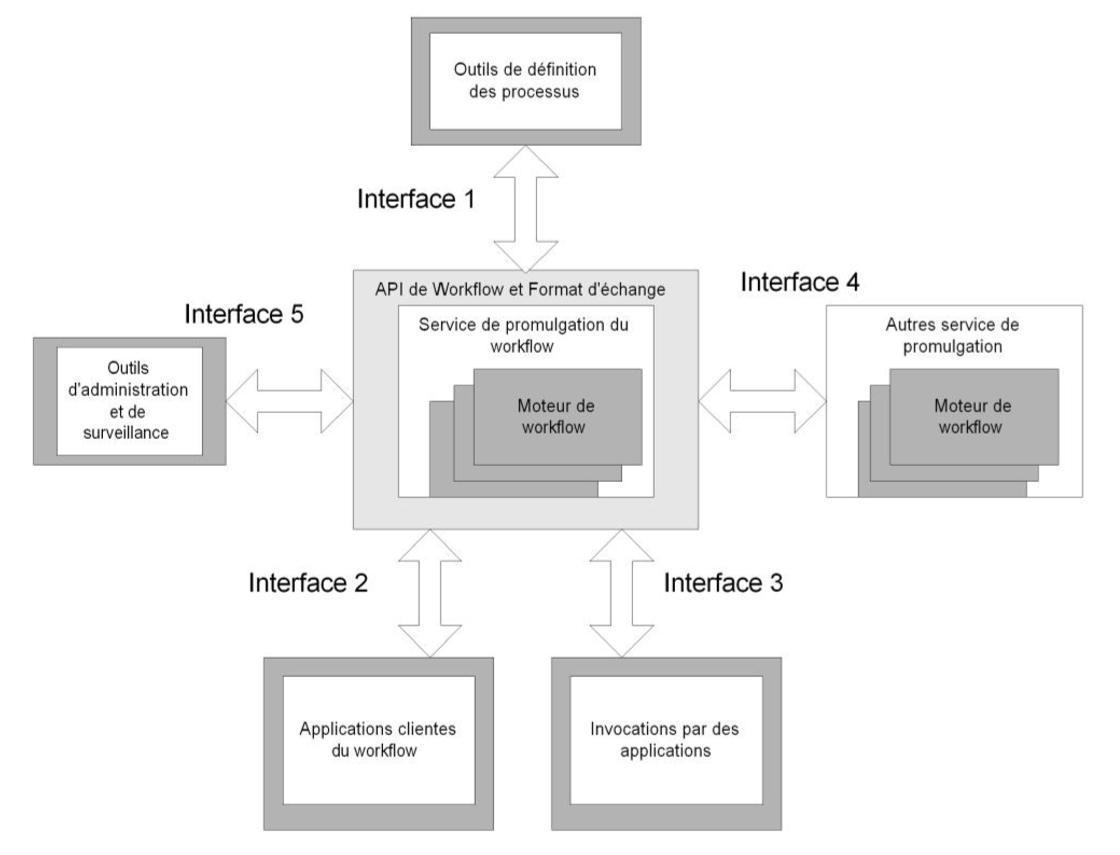
\includegraphics[width=0.6\linewidth]{Capture6}
	\caption{ Modèle de référence des systèmes de gestion de workflow (WfMC, 95). }
	\label{fig:capture6}
\end{figure}


\subsubsection{Interface avec les Outils de définition de procédures }
Cette interface, située entre les outils de modélisation/définition et le logiciel de gestion
du Workflow pendant l’exécution, est nommée interface d’import/export de définition de processus. Cette interface définit le format d’échange et d’appels des APIs, qui permettent
l'échange d'informations de définition de procédures sur une variété de médias d'échange :
physiques ou électroniques. Cette interface permet l'échange d'une définition de processus
complète ou d’un sous-ensemble. Par exemple le changement de définition d’un ensemble de
procédures ou plus simplement la modification des attributs d'une activité particulière dans
une définition de procédures. 

\subsubsection{Interface avec les applications clientes Workflow }
La liste des tâches (Worklist) à exécuter par une ressource est généralement définie et gérée par le service d’exécution du Workflow. Cette liste doit pouvoir déclencher des appels à
des applications clientes diverses et des ressources. La solution retenue pour respecter la susdite exigence, consiste à encapsuler la variété d’application qui peut être utilisée derrière un jeu standard d'API (le WAPI Workflow Application Programming interface). Ce jeu permet ainsi d’utiliser une communication standardisée entre les applications clientes, le moteur de Workflow et les Worklist, indifféremment de la nature de l’implémentation réelle des produits
clients. 
\subsubsection{Interface avec les applications invoquées}
Il est évident que le système Workflow ne peut pas intégrer l’invocation automatique de
toutes les applications qu’il peut être amené à utiliser pendant l’exécution d’un Workflow. Par
exemple les applications dont les données sont fortement typées. Dans ce cas un composant
externe supplémentaire, nommé agent d’application, est ajouté, il est chargé de la traduction
des informations dans un format compréhensible par le standard WAPI. 

Dans le cas le plus simple, l'invocation d'application est traitée localement par un moteur
de Workflow, mais les applications invoquées peuvent être utilisées par plusieurs moteurs de
Workflow et peuvent se situer sur des machines distantes, il convient donc de définir un format commun d’utilisation des ces applications entre les Workflow dans le but de communiquer correctement et de synchroniser l’appel à ces applications. 

\subsubsection{Interface avec les autres Workflow }
Un des objectifs de la normalisation dans la définition de Workflow est de pouvoir
transmettre des WorkItem entre deux systèmes Workflow conçus par des concepteurs de systèmes Workflow différents. Trois principaux types d’interopérabilité ont étés identifiés : 

\textbf{Workflow chaînés :} La dernière activité d’un Workflow A doit pouvoir fournir un item à la première activité d’un Workflow B.

\textbf{ Workflow hiérarchiques :} une activité d’un Workflow A doit pouvoir être vu comme un
 Workflow B. 
 
 \textbf{Workflow Peer to Peer :} Une procédure globale est composée d’activités gérées en partie par un Workflow et en partie par un autre Workflow, sans système de supervision de
 la procédure complète. 
 
 \textbf{Workflow Synchronisés :} Deux Workflow s’exécutent en parallèle et doivent pouvoir se
 synchroniser sur certaines activités. 
 
 Pour résumer, il est possible d’identifier deux aspects principaux nécessaires à
 l’inter fonctionnement de Workflow :

 • L’interprétation commune de la définition de procédures (ou d’un sous-ensemble).
 
 • L’appui pendant l'exécution de l’échange des divers types d'information de contrôle et
 le transfert des données appropriées et/ou d'applications entre les services d’exécution Workflow différents.
 
 \subsubsection{Interface avec les outils de contrôle et d’administration }


L’objectif de cette interface est de permettre à un logiciel de Monitoring de Workflow de
s’interfacer avec plusieurs Workflow différents et ainsi regrouper la supervision d’un ensemble de systèmes Workflow dans un logiciel.


L'interface 5 permet à une application de gestion indépendante d’interagir avec des
Workflow de différents domaines. L'application de gestion peut aussi se charger d'autres fonctions de gestion, au-delà de celles-ci. Par exemple, elle peut aussi gérer des définitions de procédures de Workflow, agissant comme un dépôt d’information commun à plusieurs systèmes
et distribuant des définitions de processus aux divers Workflow via des opérations au travers
de leurs interfaces 1.
Malgré cela, des scénarii d’implémentations moins modulaires sont aussi envisageables;
par exemple l'application de gestion peut être une partie intégrante du service d’exécution.  
 
 
 
 
\subsubsection{Standards utilisés dans les SGWf :}

\begin{figure}[!h]
	\centering
	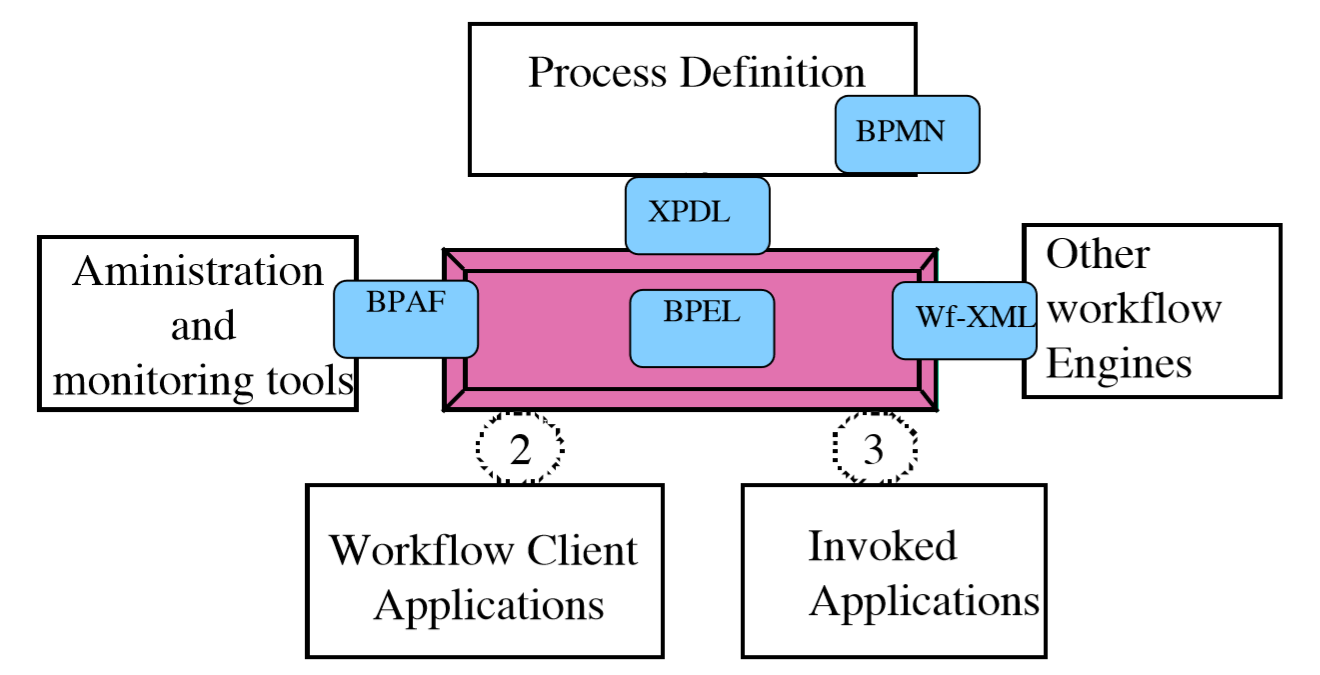
\includegraphics[width=0.6\linewidth]{Capture7}
	\caption{Différents standards adoptés dans les SGWf}
	\label{fig:capture7}
\end{figure}


\begin{enumerate}
\item \textbf{ BPNM (Business Process Model and Notation):} est une représentation graphique permettant de spécifier les processus métier maintenus par le groupe de gestion d'objets (OMG). 
\item \textbf{XPDL (Process Definition Language):} est un format normalisé par la WfMC (Workflow Management Coalition) pour l’échange de définitions de partenaire entre différents produits de flux de travail, c.-à-d. entre différents outils de modélisation et suites de gestion. XPDL définit un schéma XML pour spécifier la partie déclarative du workflow / partenaire.
\item \textbf{BPAF (Business Process Analytics):} fournit aux participants aux processus et aux décideurs des informations sur l'efficacité des processus organisationnels.
\item \textbf{BPEL (Business Process Execution Language):} BPEL est un langage d'orchestre.
\item \textbf{ Wf-XML }est un standard BPM développé par la Workflow Management Coalition. Wf-XML offre à un moteur BPM un moyen standard d'appeler un processus dans un autre moteur BPM et d'attendre qu'il se termine.
\end{enumerate}
 

\subsection{ Intérêt du cloud pour les workflows }
Les clouds offrent plusieurs avantages pour les applications à base de workflows. 
Ces avantages facilitent: 
\subsubsection{L’approvisionnement de ressources }
Dans les grilles, l'ordonnancement est basé sur un modèle en best-effort, dans lequel l’utilisateur spécifie la quantité de temps nécessaire et délègue la responsabilité de l'allocation des ressources et d'ordonnancement de tâches à un ordonnanceur fonctionnant en mode batch utilisant des files d’attentes. Dans le cloud, au lieu de déléguer l’allocation au gestionnaire de ressources, l'utilisateur peut provisionner les ressources nécessaires et ordonnancer les tâches en utilisant un ordonnanceur contrôlé par l'utilisateur. Ce modèle d’approvisionnement est idéal pour les workflows, car il permet au système de gestion de workflow d'allouer une ressource une seule fois et de l'utiliser pour exécuter de nombreuses tâches. 
\subsubsection{L’allocation dynamique de ressources à la demande }
Contrairement aux grilles, les clouds donnent l'illusion que les ressources informatiques disponibles sont illimitées. Cela signifie que les utilisateurs peuvent demander, et s’attendre à obtenir des ressources suffisantes pour leurs besoins, à tout moment. L’approvisionnement à la demande est idéal pour les workflows et d'autres applications faiblement couplées, car il réduit le surcoût (overheads) d’ordonnancement total et peut améliorer considérablement les performances du workflow (Singh, 2005 ; Juve, 2008) 
\subsubsection{L’élasticité}
Outre l’approvisionnement des ressources à la demande, les clouds permettent aussi aux utilisateurs de libérer des ressources à la demande. La nature élastique de clouds facilite le changement des quantités et des caractéristiques de ressources lors de l'exécution, permettant ainsi d’augmenter le nombre de ressources, quand il y a un grand besoin, et d’en diminuer, lorsque la demande est faible. Cela permet aux systèmes de gestion de workflow de répondre facilement aux exigences de qualité de service (QoS) des applications, contrairement à l'approche traditionnelle, qui nécessite de réserver à l'avance des ressources dans les environnements de grilles. 
\subsubsection{La garantie des QoS via des SLA }
Avec l’arrivée des services de cloud computing  provenant de grandes organisations commerciales, les accords de niveau de service (SLA) ont été une préoccupation importante pour les fournisseurs et les utilisateurs. En raison de compétitions entres les fournisseurs de services émergents, un grand soin est pris lors de la conception du SLA qui vise à offrir (i) de meilleures garanties de QoS aux utilisateurs, et (ii) des termes clairs pour l'indemnisation, en cas de violation du contrat. Cela permet aux systèmes de gestion de workflow de fournir de meilleures garanties de bout en bout en "mappant" les utilisateurs aux fournisseurs de services selon les caractéristiques des SLA.

\subsubsection{Le faible Coût d’exploitation }
 Économiquement motivés, les fournisseurs de cloud commercial s'efforcent d'offrir de meilleures garanties de services par rapport aux fournisseurs de grille. Les fournisseurs de cloud profitent également des économies d'échelle, en fournissant des ressources de calcul, de stockage et de bande passante, à un coût très faible grâce, à la virtualisation. Ainsi l'utilisation des services de cloud public pourrait être économique et une alternative moins coûteuse, par rapport à l’utilisation de ressources dédiées, qui sont plus chères. Un des avantages de l'utilisation des ressources virtuelles pour l'exécution de workflow, plutôt que d'un accès direct à la machine physique, est le besoin réduit pour sécuriser les ressources physiques des codes malveillants. Cependant, l'effet à long terme de l'utilisation de ressources virtuelles dans les clouds qui partagent efficacement une "tranche" de la machine physique, plutôt que d'utiliser des ressources dédiées pour les workflows de calculs intensifs, est une question de recherche intéressante. 
\section{Conclusion}
....lk
